\documentclass[10pt,a4paper]{article}
\usepackage[margin=2cm]{geometry}
\usepackage[utf8]{inputenc}
\usepackage[LGR,T1]{fontenc}
\usepackage{lmodern}
\usepackage{textalpha}
\usepackage{substitutefont}
\substitutefont{LGR}{\rmdefault}{cmr}
\substitutefont{LGR}{\sfdefault}{cmss}
\substitutefont{LGR}{\ttdefault}{cmtt}
\usepackage{textcomp}
\sloppy\emergencystretch=3em
\usepackage{amsmath,graphicx,booktabs,xcolor,enumitem,array,float}\usepackage[hidelinks]{hyperref}
\setlength{\parskip}{0.45em}\setlength{\parindent}{0pt}\setlist{itemsep=0.1em,topsep=0.2em}
\newcommand{\ptr}[1]{{\footnotesize\texttt{#1}}}
\title{QRL-Lab: είσοδος, αποτελέσματα και αρχιτεκτονικές των μοντέλων\\\large cycle 3 \textperiodcentered{} batch S \textperiodcentered{} workload \texttt{poisson\_ms\_spiky} (και shift)}
\author{Πάρις --- ετοιμάστηκε για τον Κώστα (M-20261110-003, J444)}\date{10/11/2026}
\begin{document}\maketitle
\section{Τι περιέχει και τι ΟΧΙ}
\begin{itemize}
\item Όλα τα νούμερα είναι \textbf{validation} (spiky: val 16000--16019, shift: val 13500--13509)\textperiodcentered{} \textbf{κανένα test split} δεν χρησιμοποιήθηκε, καμία νέα εκπαίδευση. Δεν είναι συμπέρασμα γενίκευσης ούτε claim.
\item Τα σχήματα adaptation (pods vs load) προέρχονται από \textbf{eval-only} επανεκτέλεση των αποθηκευμένων checkpoints του training seed 19100 (ένα seed ανά μοντέλο) σε 3 val επεισόδια (seeds 16000--16002), μέσω \ptr{tools/envelope.py} (envelope cycle3). Άρα δείχνουν συμπεριφορά ενός εκπαιδευμένου μοντέλου, όχι μέσο όρο seeds.
\item Το RPPO/DRe-SCale έχει δικό του module (\ptr{tuning/rppo.py}) χωρίς καταγραφή τροχιάς\textperiodcentered{} ΔΕΝ υπάρχει σχήμα pods-vs-load γι' αυτό (τα νούμερα return και η αρχιτεκτονική υπάρχουν). Δεν επινοήθηκε τίποτα.
\item Το latency είναι \emph{proxy} (χρόνος παραμονής στην ουρά + $l_0$ τη στιγμή της αποδοχής), όχι μετρημένος χρόνος απόκρισης (\ptr{tuning/poisson\_ms.py}, docstring).
\item Οι αρχιτεκτονικές διαβάστηκαν από τον κώδικα και από τα \texttt{.pt} checkpoints\textperiodcentered{} ο αριθμός παραμέτρων μετράται από τα state\_dict (συμφωνεί με \texttt{n\_params} των JSON).
\end{itemize}

\section{Είσοδος: workload και μετρικές}
Περιβάλλον: ουρά αιτημάτων με πόδια (pods) 1--20, $\mu=10$ αιτήματα/pod/tick, καθυστέρηση εκκίνησης pod 5 ticks, ουρά max 200, SLO: p95 latency $>1.0$ ή drops, κόστος pod 3/tick, ποινή SLO 20, ποινή drop 1 ανά αίτημα, επεισόδιο 5000 ticks, αρχικά 6 pods. Ρυθμός: $\lambda_t=\text{base}\cdot(1+0.4\sin(2\pi t/1000+\varphi))\cdot e^{x_t}$ (AR(1) log-noise, $\phi=0.98$, $\sigma=0.15$), $N_t\sim\text{Poisson}(\lambda_t)$. Η \texttt{spiky} παραλλαγή αντικαθιστά τη μαρκοβιανή έκρηξη με επικάλυψη γεγονότων (απότομα flash-crowds, ράμπες, ριπές), με $\lambda\le190$. Η \texttt{shift} έχει συχνότερες εκρήξεις ($r_{nb}=1/300$) και $\sigma=0.30$. Δράσεις: 0 κάτω / 1 μένω / 2 πάνω. Reward $=\text{served}-3\cdot\text{pods}-20\cdot[\text{SLO}]-\text{drops}$. \ptr{code-poisson-c345/tuning/poisson\_ms.py:1-34,55-124}.

State 7 διαστάσεων: [arrivals, capacity, CPU\%, mem\%, p95 latency, active pods, pending pods]\textperiodcentered{} κανονικοποίηση (obs\_scale) με διαιρέτες 100,100,100,100,2,20,20 και reward/10 (\ptr{S/c3S-dinos-s19100.json}).
\begin{figure}[htbp]\centering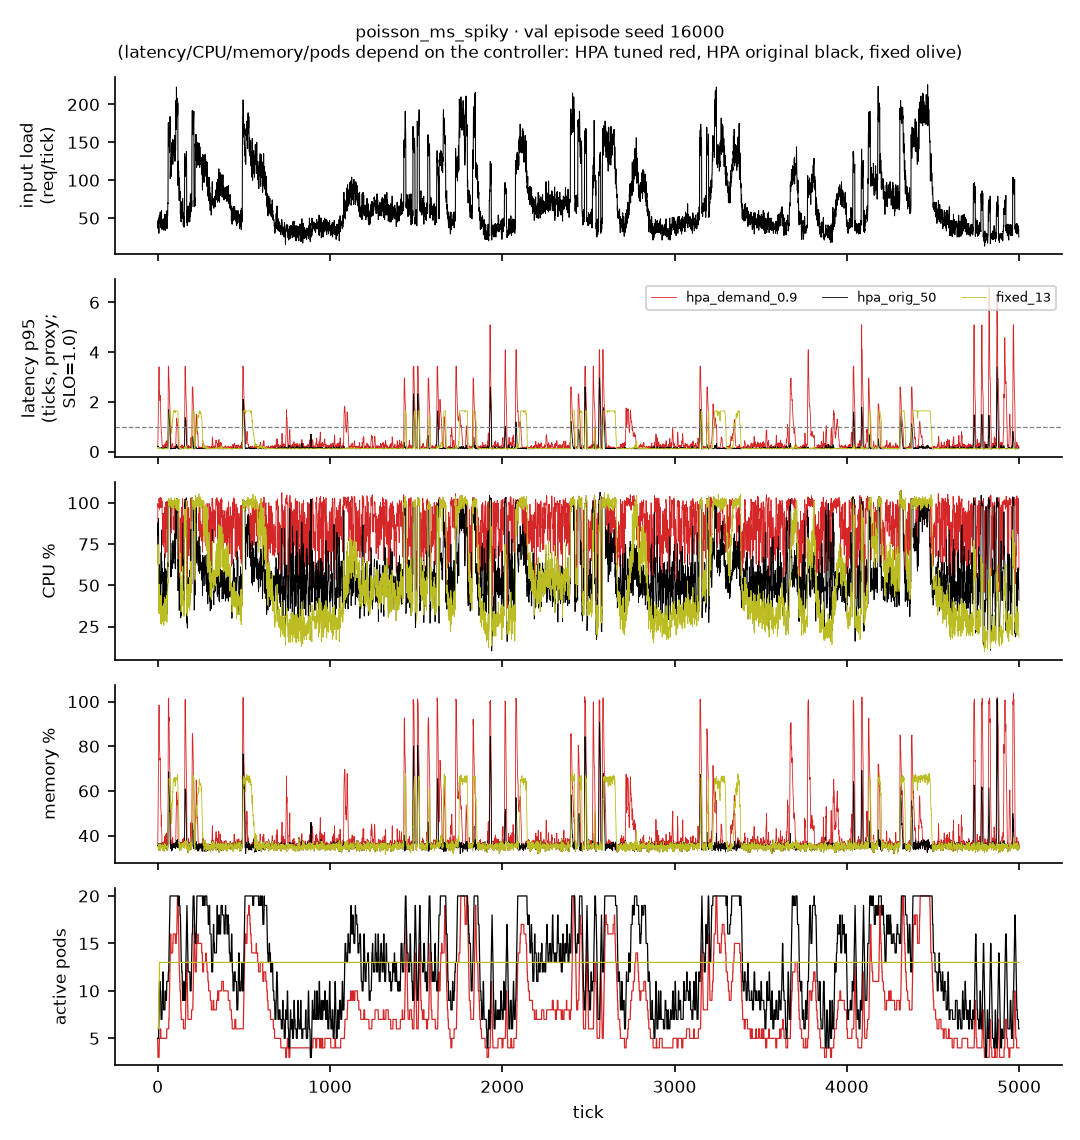
\includegraphics[width=1.0\linewidth,height=0.8\textheight,keepaspectratio]{fig/workload_spiky.png}\par\small Είσοδος (spiky, val seed 16000): load και, για τρεις ελεγκτές αναφοράς, latency p95, CPU, μνήμη και pods. Τα CPU/mem/latency εξαρτώνται από τον ελεγκτή\textperiodcentered{} δεν είναι ιδιότητα της εισόδου μόνο. Πηγή: eval-only \ptr{base\_spiky.json}.\end{figure}
\begin{figure}[htbp]\centering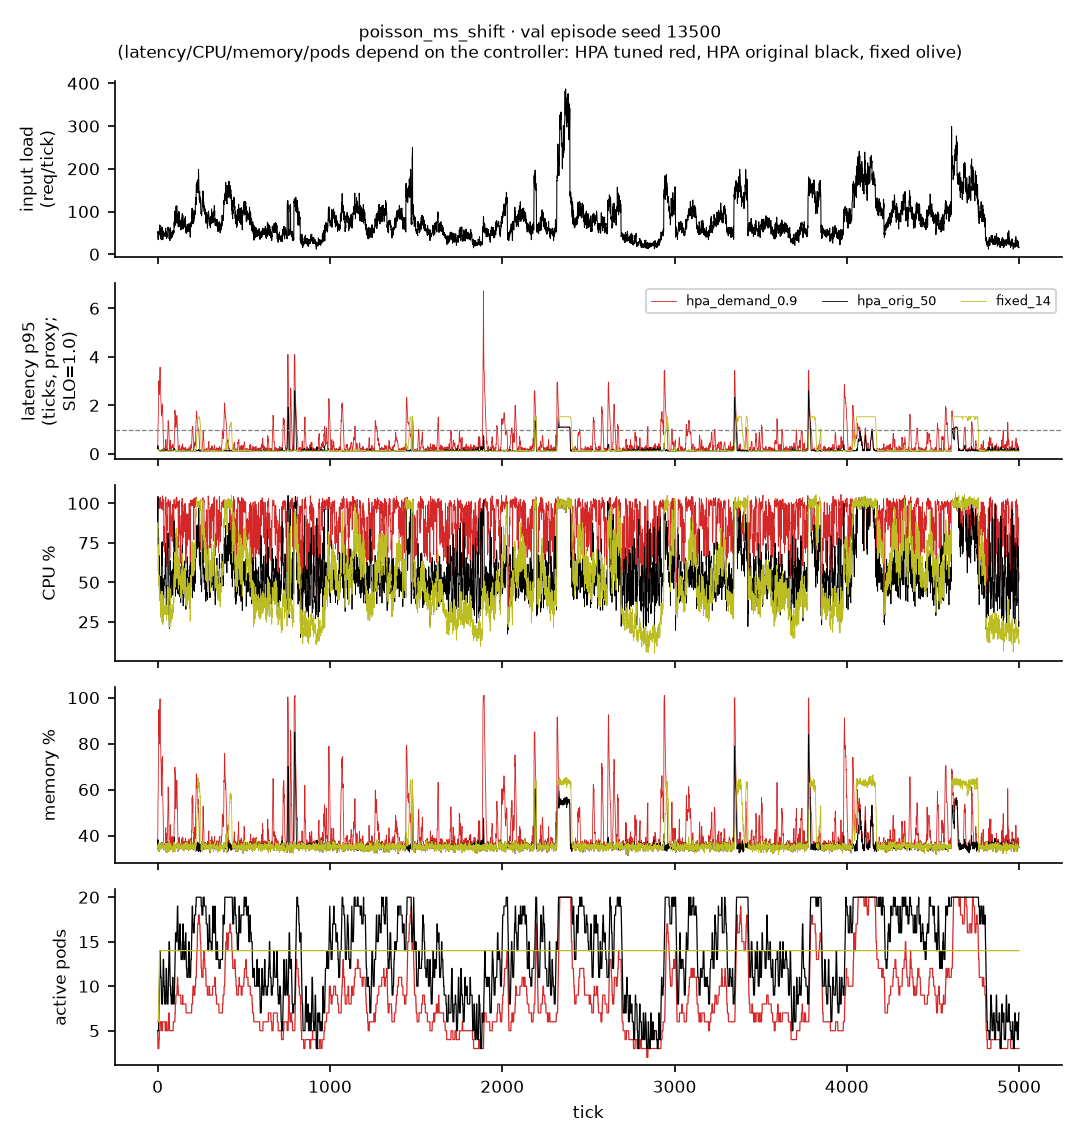
\includegraphics[width=1.0\linewidth,height=0.8\textheight,keepaspectratio]{fig/workload_shift.png}\par\small Ίδιο για το shift workload (val seed 13500).\end{figure}

\section{Συνολικό reward ανά μοντέλο}
\begin{figure}[htbp]\centering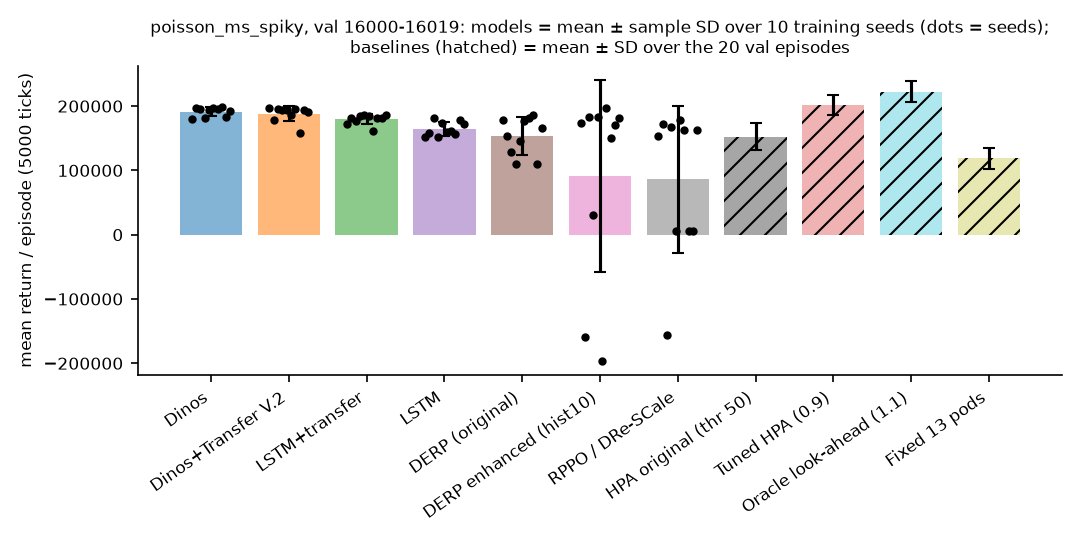
\includegraphics[width=1.0\linewidth,height=0.8\textheight,keepaspectratio]{fig/rewards_spiky.png}\par\small Return ανά επεισόδιο, spiky val. Μοντέλα: μέσο ± sample SD των 10 training seeds 19100--19109 (μία κουκκίδα ανά seed, μέσος 20 val επεισοδίων, ένα checkpoint 19968 ticks). Baselines: μέσο ± SD των 20 val επεισοδίων με παραμέτρους επιλεγμένες στο ίδιο val (P0)\textperiodcentered{} δεν είναι ανεξάρτητα από το val.\end{figure}

\begin{table}[H]\centering\footnotesize\begin{tabular}{lrrrrrrr}\toprule
Μοντέλο & μέσο & SD & διάμεσος & min seed & max seed & SLO viol. & παράμετροι\\\midrule
Dinos & 191.600 & 7.100 & 194.839 & 179.310 & 198.179 & 0.106 & 104.451 \\
Dinos+Transfer V.2 & 188.131 & 12.028 & 193.814 & 157.622 & 196.609 & 0.103 & 104.451 \\
LSTM+transfer & 179.877 & 7.668 & 182.139 & 161.564 & 186.441 & 0.145 & 334.723 \\
LSTM & 164.648 & 10.901 & 160.015 & 152.236 & 181.322 & 0.224 & 334.723 \\
DERP (original) & 153.579 & 29.403 & 159.519 & 109.306 & 186.855 & 0.048 & 17.923 \\
DERP enhanced (hist10) & 91.481 & 149.827 & 172.010 & -196.017 & 197.699 & 0.355 & 25.987 \\
RPPO / DRe-SCale & 86.009 & 113.946 & 158.219 & -155.721 & 178.669 & 0.386 & 584.196 \\
\midrule
HPA original (thr 50) & 152.439 & 20.709 & \multicolumn{3}{c}{20 val episodes} & -- & -- \\
Tuned HPA (0.9) & 201.856 & 15.482 & \multicolumn{3}{c}{20 val episodes} & -- & -- \\
Oracle look-ahead (1.1) & 222.674 & 17.020 & \multicolumn{3}{c}{20 val episodes} & -- & -- \\
Fixed 13 pods & 119.208 & 16.259 & \multicolumn{3}{c}{20 val episodes} & -- & -- \\
\bottomrule\end{tabular}
\caption{Πηγή: \ptr{.lab/j442/summary.json} (μοντέλα), \ptr{code-poisson-spiky/tuning/results/spiky-stage1/spiky1-P0-reference-off-s16000.json} (baselines). Ο oracle είναι look-ahead ευρετικός, όχι άνω φράγμα (\ptr{docs/paper\_notes.md} §6).}\end{table}
Παρατηρήσεις (περιγραφικά): όλα τα μοντέλα είναι κάτω από το tuned HPA (201,9k) και τον oracle (222,7k)\textperiodcentered{} Dinos και Dinos+Transfer V.2 δεν διακρίνονται (paired διαφορά $-3{,}5\text{k}\pm16{,}9\text{k}$, \ptr{.lab/j442}). DERP enhanced και RPPO είναι ασταθή (seeds με αρνητικό return).
\begin{figure}[htbp]\centering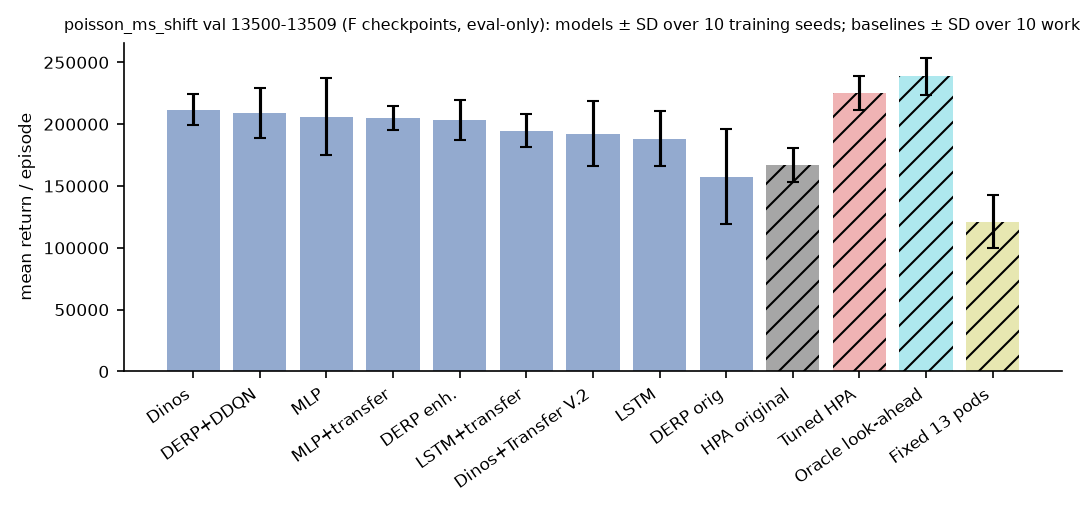
\includegraphics[width=1.0\linewidth,height=0.8\textheight,keepaspectratio]{fig/rewards_shift.png}\par\small Shift workload (held-out), τα checkpoints F (10 seeds, 39936 ticks) αξιολογημένα eval-only στο val. Πηγή: \ptr{.lab/j438/summary.json}. Περιγραφικό, όχι test.\end{figure}

\section{Προσαρμογή: pods ως προς το load}
\begin{figure}[htbp]\centering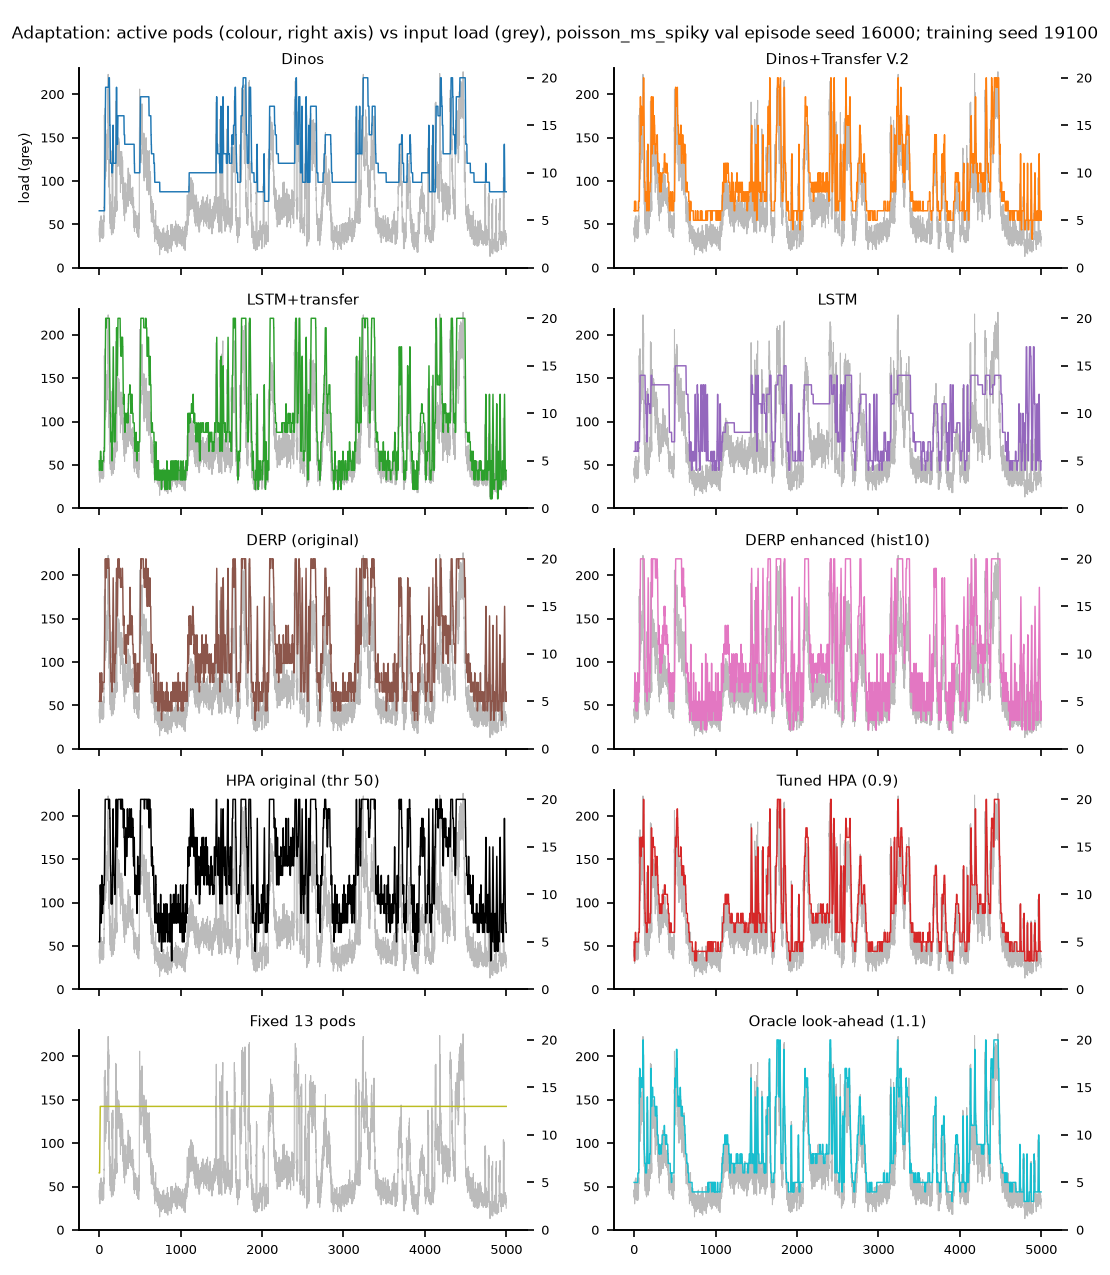
\includegraphics[width=1.0\linewidth,height=0.8\textheight,keepaspectratio]{fig/adaptation_timeseries.png}\par\small Pods (έγχρωμο, δεξιός άξονας) και load (γκρι) στο ίδιο val επεισόδιο, ένα training seed (19100) ανά μοντέλο\textperiodcentered{} στο τέλος οι ελεγκτές αναφοράς.\end{figure}
\begin{figure}[htbp]\centering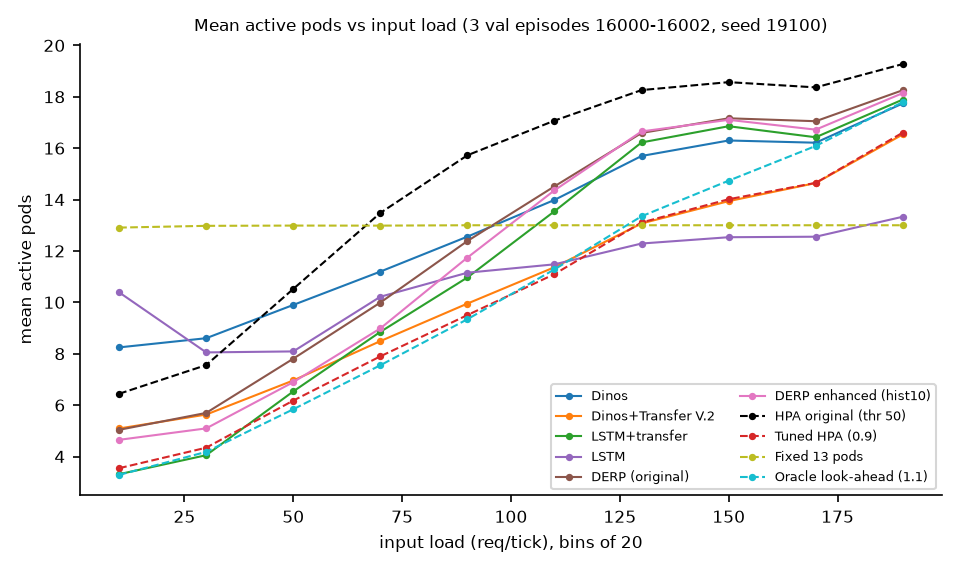
\includegraphics[width=0.85\linewidth,height=0.8\textheight,keepaspectratio]{fig/adaptation_pods_vs_load.png}\par\small Μέσος αριθμός pods ανά κλάση load. Ένα training seed, 3 val επεισόδια.\end{figure}

\section{Αρχιτεκτονικές των μοντέλων}
Κοινά (αν δεν αναφέρεται διαφορετικά): 3 δράσεις, reward/10, κανονικοποιημένη είσοδος 7 χαρακτηριστικών, Adam, απώλεια SmoothL1 (Huber), Double DQN (online argmax / target τιμή, detached) για τους LSTM arms, replay από μνήμη, 16 διαδοχικές ενημερώσεις ανά replay, ένα replay ανά tick όταν η μνήμη $>16$. Παράθυρο ιστορικού 10 ticks για τα LSTM. Training 19968 ticks target (transfer: 9984 pretrain + 9984 finetune, συνολικά 19968). Πηγές: \ptr{tuning/legacy/\{network\_dense,networks\_lstm,agent\_lstm\_fixed,agent\_lstm\_v2,ddqnagent,c5\_protocol\}.py}, \ptr{tuning/rppo.py}, και τα JSON του batch S \ptr{tuning/results/cycle3/S/}.
\begin{table}[H]\centering\scriptsize\setlength{\tabcolsep}{3pt}\begin{tabular}{p{2.4cm}p{3.9cm}rp{1.1cm}rrrrp{1.4cm}}\toprule
Μοντέλο & Δίκτυο & params & lr & batch & γ & replay & n-step & target sync\\\midrule
DERP original & MLP 7-128-128-3 & 17.923 & $10^{-4}$ & 16 & 0.95 & 500 & -- & κάθε replay\\
DERP enhanced & MLP 70-128-128-3 & 25.987 & $10^{-4}$ & 16 & 0.95 & 500 & -- & κάθε replay\\
LSTM & 3$\times$LSTM(128)+FC & 334.723 & $10^{-4}$ & 16 & 0.98 & 5000 & 2 & 100\\
LSTM+transfer & 3$\times$LSTM(128)+FC & 334.723 & $10^{-4}$ & 16 & 0.98 & 5000 & 1 & 250\\
Dinos & LSTM128 $\to$ concat $\to$ 128 $\to$ 128 & 104.451 & $5\cdot10^{-5}$ & 16 & 0.98 & 5000 & 3 & 100\\
Dinos+Transfer V.2 & ίδιο με Dinos & 104.451 & $10^{-4}$ & 16 & 0.98 & 5000 & 5 & 250\\
RPPO / DRe-SCale & LSTM256 + MLP 64-64 (actor, critic) & 584.196 & $3\cdot10^{-4}$ & 128 & 0.99 & rollout 128 & -- & -- \\\bottomrule\end{tabular}
\caption{Σύνοψη. Πηγές: JSON του S (\texttt{hyperparameters}, \texttt{ddqn\_options}, \texttt{target\_sync\_replays}, \texttt{learning\_rate}), \ptr{ddqnagent.py:15-30}, \ptr{agent\_lstm\_fixed.py:1-16,153-154}, \ptr{rppo.py:1-13,44-45}. Το batch size των DQN arms είναι τα 16 δείγματα ανά replay (\ptr{run\_legacy.py:127}); το «batch» του RPPO είναι ολόκληρο το rollout των 128 βημάτων.}\end{table}

\subsection{DERP (original) --- \texttt{derp}}
Πυκνό δίκτυο: \texttt{fc1} Linear(7,128) $\to$ ReLU $\to$ \texttt{fc2} Linear(128,128) $\to$ ReLU $\to$ \texttt{fc3} Linear(128,3) (Q-τιμές των 3 δράσεων). Πλήρως συνδεδεμένα (fully connected), χωρίς μνήμη: βλέπει μόνο την τρέχουσα παρατήρηση. 17.923 παράμετροι. Αλγόριθμος: DDQN του αρχικού DInos (verbatim port), μνήμη 500, $\gamma=0.95$, Adam $10^{-4}$, SmoothL1, replay(16) κάθε tick. $\epsilon$: γραμμικά 1$\to$0.01 σε 10k ticks (\texttt{linear10k}, \texttt{epsilon\_min}=0.01 στο JSON). Στόχος: $r+\gamma\max_a Q_{\text{target}}(s',a)$ όπως στο αρχικό\textperiodcentered{} στο S δεν ενεργοποιείται double/n-step. Χωρίς transfer.

\subsection{DERP enhanced --- \texttt{derp\_hist10}}
Ίδιο δίκτυο, αλλά είσοδος η ισοπεδωμένη ιστορία 10 παρατηρήσεων (10$\times$7=70): Linear(70,128)$\to$ReLU$\to$Linear(128,128)$\to$ReLU$\to$Linear(128,3), 25.987 παράμετροι. $\epsilon$: πολλαπλασιαστικά $\times$0.995 ανά replay (\texttt{eps\_schedule=original}), ελάχιστο 0.01. Άλλα ίδια με το DERP. Ασταθές στο S (SD 149,8k).

\subsection{LSTM --- \texttt{lstm\_scratch}, variant \texttt{fixed}}
Αναδρομικό δίκτυο (LSTM) \texttt{myLSTM}: είσοδος παράθυρο [10$\times$7] $\to$ 3 στοιβαγμένα επίπεδα LSTM με 128 κρυφούς νευρώνες το καθένα (τα $h,c$ ξεκινούν από μηδέν σε κάθε παράθυρο) $\to$ η έξοδος του τελευταίου tick $\to$ Linear(128,3). Σύνδεση: μέσα στο κάθε επίπεδο οι νευρώνες συνδέονται με πύλες (input, forget, cell, output) και αναδρομικές συνδέσεις\textperiodcentered{} τα επίπεδα συνδέονται σειριακά. 334.723 παράμετροι. Double DQN με n-step 2, $\gamma=0.98$, μνήμη 5000, 16 ενημερώσεις ανά replay, target sync κάθε 100 replays, lr $10^{-4}$, $\epsilon$ 1$\to$0.05 γραμμικά σε 10k ticks.

\subsection{LSTM+transfer --- \texttt{dinos\_t}, variant \texttt{fixed}}
Ίδιο δίκτυο με το LSTM. Pretraining 9984 ticks στο \texttt{spike300\_d5} (cycle-1 περιβάλλον, ίδιο μέγεθος state), μετά finetune 9984 ticks στο \texttt{poisson\_ms\_spiky} με επανεκκίνηση $\epsilon$ (restart). n-step 1, target sync 250, lr $10^{-4}$. Ο αριθμός παραμέτρων είναι ίδιος (334.723).

\subsection{Dinos --- \texttt{lstm\_scratch}, variant \texttt{a1h}}
«Dinos V.2-H»: \texttt{window[10$\times$7] $\to$ LSTM(7,128, 1 επίπεδο, μηδενικά $h,c$ ανά παράθυρο) $\to$ concat(τελευταία έξοδος[128], τελευταία παρατήρηση[7]) $\to$ Dense(135,128) ReLU $\to$ Dense(128,128) ReLU $\to$ Dense(128,3)} (πεδίο \texttt{architecture} του JSON). Δηλαδή ένα LSTM που συνοψίζει την ιστορία, ενώνεται (skip σύνδεση) με την τρέχουσα παρατήρηση και περνά από 3 πυκνά επίπεδα. 104.451 παράμετροι. Double DQN, n-step 3, $\gamma=0.98$, μνήμη 5000, 16 ενημερώσεις/replay, target sync 100 replays, Adam lr $5\cdot10^{-5}$, gradient clipping max-norm 10, $\epsilon$ 1$\to$0.05 σε 10k ticks. Χωρίς pretraining. Σημείωση: το grad-clip ενεργοποιείται σχεδόν πάντα (clip\_frac 0,988 στο seed 19100, \ptr{c3S-dinos-s19100.json}, \texttt{grad\_norm}).

\subsection{Dinos+Transfer V.2 --- \texttt{dinos\_t}, variant \texttt{a1h}}
Ίδια αρχιτεκτονική με το Dinos (104.451 παράμετροι)\textperiodcentered{} η διαφορά είναι στην εκπαίδευση: pretraining 9984 ticks στο ίδιο workload \texttt{poisson\_ms\_spiky}, μετά finetune 9984 ticks με restart του $\epsilon$ (συνολικά 19968)\textperiodcentered{} n-step 5, target sync 250, lr $10^{-4}$, χωρίς grad-clip στο JSON (\texttt{hyperparameters}). Ονομασία πάντα «Dinos+Transfer V.2».

\subsection{RPPO / DRe-SCale --- \texttt{rppo}}
Recurrent PPO (native torch υλοποίηση, \ptr{tuning/rppo.py}, όπως οι προεπιλογές sb3\_contrib): δύο ξεχωριστά LSTM 256 νευρώνων (ένα για τον actor, ένα για τον critic, \texttt{lstm\_pi}, \texttt{lstm\_vf}, είσοδος 7), μετά MLP [64,64] με Tanh ανά κλάδο, κεφαλή πολιτικής Linear(64,3) (κατηγορική κατανομή) και κεφαλή τιμής Linear(64,1). 584.196 παράμετροι. Hyperparameters (JSON): n\_steps 128, batch 128 (ένα minibatch ανά rollout), n\_epochs 10, lr $3\cdot10^{-4}$ (Adam, eps $10^{-5}$), $\gamma=0.99$, GAE $\lambda=0.9$, clip 0.2, ent\_coef 0, vf\_coef 0.5, max\_grad\_norm 0.5, ορθογώνια αρχικοποίηση. On-policy\textperiodcentered{} αξιολόγηση με greedy (argmax) πολιτική. Ασταθές στο S.

\section{Αναπαραγωγή και όρια}
Αριθμοί: \ptr{.lab/j442/summary.json}, \ptr{.lab/j438/summary.json}\textperiodcentered{} σχήματα: \ptr{tools/j444/figs.py}, \ptr{tools/j444/build\_pdf.py}\textperiodcentered{} eval-only runs: spec \ptr{.lab/j444/spec.json} (envelope cycle3, χωρίς training, μόνο val). Ένα training seed ανά μοντέλο στα σχήματα προσαρμογής\textperiodcentered{} τα 20 val επεισόδια του return δεν έχουν καταγραφεί ανά tick. Άγνωστο/μη διαθέσιμο: τροχιά RPPO\textperiodcentered{} CPU-seconds του launcher για τα εξωτερικά runs (\texttt{cpu\_seconds: None}).
\end{document}
